%%========================================================================
%% LaTeX sjabloon voor bachelorproef toegepaste informatica
%%  HoGent Bedrijf en Organisatie - Bijlagenbundel
%%========================================================================

%%========================================================================
%% Preamble
%%========================================================================

\documentclass[pdftex,a4paper,12pt,twoside]{report}

% XXX: Let op: dit sjabloon is gemaakt om dubbelzijdig af te drukken
% Voor enkelzijdig, verwijder ``twoside'' hierboven.

%%---------- Extra functionaliteit ---------------------------------------

\usepackage[utf8]{inputenc}  % Accenten gebruiken in tekst (vb. é ipv \'e)
\usepackage{amsfonts}        % AMS math packages: extra wiskundige
\usepackage{amsmath}         %   symbolen (o.a. getallen-
\usepackage{amssymb}         %   verzamelingen N, R, Z, Q, etc.)
\usepackage[dutch]{babel}    % Taalinstellingen: woordsplitsingen,
                             %  commando's voor speciale karakters
                             %  ("dutch" voor NL)
\usepackage{eurosym}         % Euro-symbool €
\usepackage{geometry}
\usepackage{graphicx}        % Invoegen van tekeningen
\usepackage[pdftex,bookmarks=true]{hyperref}
                             % PDF krijgt klikbare links & verwijzingen,
                             %  inhoudstafel
\usepackage{listings}        % Broncode mooi opmaken
\usepackage{multirow}        % Tekst over verschillende cellen in tabellen
\usepackage{rotating}        % Tabellen en figuren roteren
\usepackage{natbib}          % Betere bibliografiestijlen
\usepackage{fancyhdr}        % Pagina-opmaak met hoofd- en voettekst

\usepackage[T1]{fontenc}     % Ivm lettertypes
\usepackage{lmodern}
\usepackage{textcomp}

\usepackage{lipsum}          % Voor vultekst (lorem ipsum)
\usepackage{pdfpages}

%%---------- Layout ------------------------------------------------------

% hoofdingen, enz.
\pagestyle{fancy}
% enkel hoofdstuktitel in hoofding, geen sectietitel (vermijd overlap)
\renewcommand{\sectionmark}[1]{}

% lijn, wordt gebruikt in titelpagina
\newcommand{\HRule}{\rule{\linewidth}{0.5mm}}

% Leeg blad
\newcommand{\emptypage}{
\newpage
\thispagestyle{empty}
\mbox{}
\newpage
}

% Gebruik een schreefloos lettertype ipv het "oubollig" uitziende
% Computer Modern
\renewcommand{\familydefault}{\sfdefault}

% Commando voor invoegen Java-broncodebestanden (dank aan Niels Corneille)
% Gebruik: \javacode{source/MijnKlasse.java}{Uitleg bij de code}
\newcommand{\javacode}[2]{ \lstset{%
  language=java,
  breaklines=true,
  float=th,
  caption={#2},
  basicstyle=\scriptsize,
  frame=single,
  extendedchars=\true
}
\lstinputlisting{#1}}

%%---------- Documenteigenschappen ---------------------------------------
%% Vul dit aan met je eigen info:

% Je eigen naam
\newcommand{\student}{Yannick Van Hecke}

% De naam van je lector, begeleider, promotor
\newcommand{\promotor}{Koen Hoof}

% De naam van je co-promotor
\newcommand{\copromotor}{Jeroen Gevenois}

% Indien je bachelorproef in opdracht van een bedrijf of organisatie
% geschreven is, geef je hier de naam.
\newcommand{\instelling}{Politiezone Gent - Dienst ICT}

% De titel van het rapport/bachelorproef
\newcommand{\titel}{Vergelijkende studie en proof-of-concept in functie van een doelbewuste keuze tussen een cross platform mobiele applicatie en een mobiele website}

% Datum van indienen
\newcommand{\datum}{2 juni 2017}

% Faculteit
\newcommand{\faculteit}{Faculteit Bedrijf en Organisatie}

% Soort rapport
\newcommand{\rapporttype}{Scriptie voorgedragen tot het bekomen van de graad van\\Bachelor in de toegepaste informatica}

% Academiejaar
\newcommand{\academiejaar}{2016-2017}

% Examenperiode
%  - 1e semester = 1e examenperiode
%  - 2e semester = 2e examenperiode
%  - tweede zit = 3e examenperiode
\newcommand{\examenperiode}{Tweede examenperiode}

%%========================================================================
%% Inhoud document
%%========================================================================

\begin{document}

%%---------- Front matter ------------------------------------------------
%% Het voorblad - Hier moet je in principe niets wijzigen.

\begin{titlepage}
  \newgeometry{top=2cm,bottom=1.5cm,left=1.5cm,right=1.5cm}
  \begin{center}

    \begingroup
    \rmfamily
    
\includegraphics[width=2.5cm]{img/HG-beeldmerk-woordmerk}\\[.5cm]
    \faculteit\\[3cm]
    \titel\\[1cm]
    Bijlagen
    \vfill
    \student\\[3.5cm]
    \rapporttype\\[2cm]
    Promotor:\\
    \promotor\\
    Co-promotor:\\
    \copromotor\\[2.5cm]
    Instelling: \instelling\\[.5cm]
    Academiejaar: \academiejaar\\[.5cm]
    \examenperiode
    \endgroup

  \end{center}
  \restoregeometry
\end{titlepage}

% Schutblad

\emptypage


\begin{titlepage}
  \newgeometry{top=5.35cm,bottom=1.5cm,left=1.5cm,right=1.5cm}
  \begin{center}

    \begingroup
    \rmfamily
    \faculteit\\[3cm]
    \titel\\[1cm]
    Bijlagen
    \vfill
    \student\\[3.5cm]
    \rapporttype\\[2cm]
    Promotor:\\
    \promotor\\
    Co-promotor:\\
    \copromotor\\[2.5cm]
    Instelling: \instelling\\[.5cm]
    Academiejaar: \academiejaar\\[.5cm]
    \examenperiode
    \endgroup

  \end{center}
  \restoregeometry
\end{titlepage}


\tableofcontents

\appendix

\chapter{Bachelorproefvoorstel}
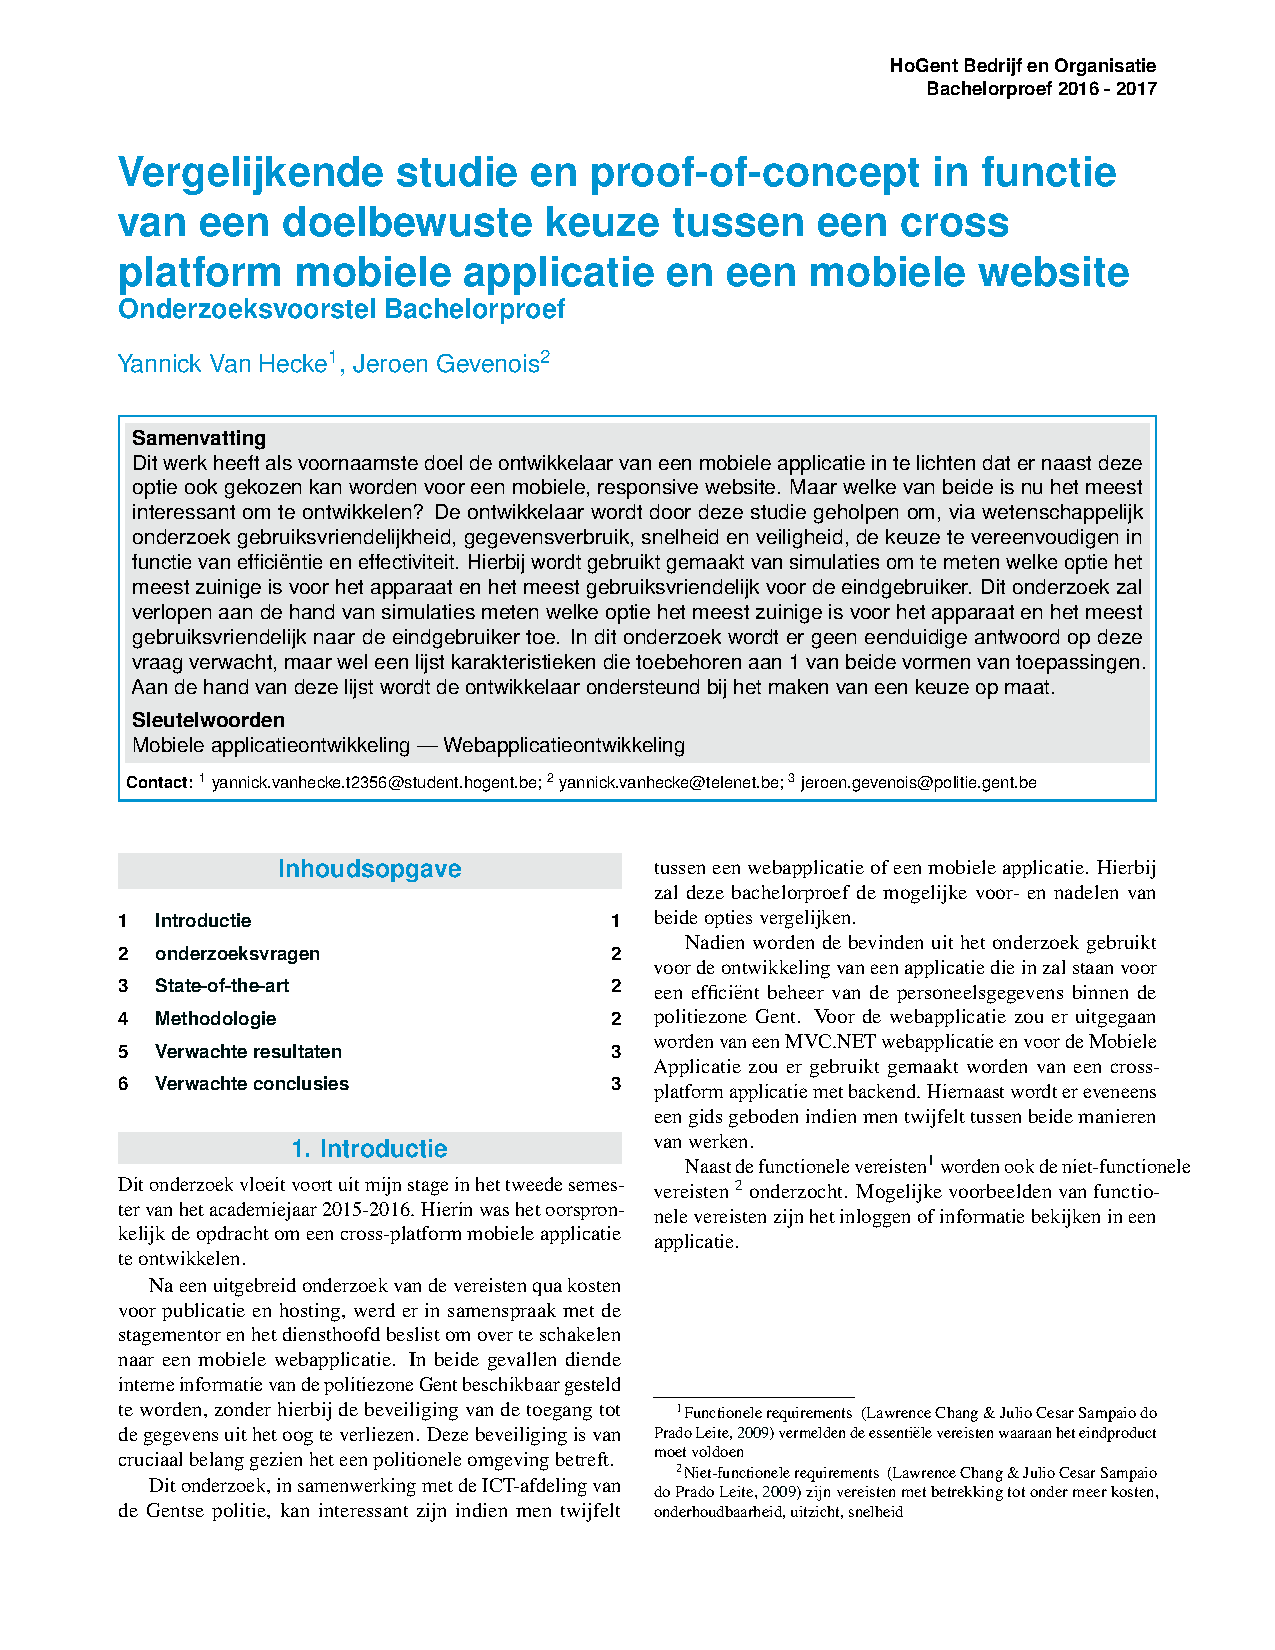
\includepdf[pages={1}]{vanhecke_yannick_voorstel.pdf}
\includepdf[pages={2}]{vanhecke_yannick_voorstel.pdf}
\includepdf[pages={3}]{vanhecke_yannick_voorstel.pdf}
\chapter{Uitgebereide resultaten ivm de ontwikkeling van de toepassingen}
\label{ch:uitgebereideresultatenmetbetrekkingtotontwikkeling}
\begin{center}
  \begin{tabular}{ | l | l | l | l | l |}
    \hline
    Functionaliteit & Android & iOS \footnote{In de iOS app is wegen gebrek aan tijd enkel het inloggen geïmplementeerd.} & Windowsphone & Webapp
    \\ \hline
    Inloggen & 7 dagen & 2 dagen & 4 dagen & 3 uur
    \\ \hline
    Overzicht & 6 dagen & nvt & 1 dag & 6 uur
    \\ \hline
    Details & 4 uur & nvt & 4 uur & 2 uur
    \\ \hline
  \end{tabular}
\end{center}


\chapter{Uitgebreide testresultaten ivm de tijden}
\label{ch:uitgebereidresultatenmetbetrekkingtottijden}

% Automatisch invoegen van al je Java broncode:
% % 1/ maak een link naar je broncodedirectory naar subdirectory source
% %      ln -s /path/to/java/src/ ./source
% %    Of kopieer desnoods al je broncodebestanden. Zorg dat je
% %    versiebeheersysteem deze directory negeert!
% % 2/ Genereer source.tex met het script source.sh
% %      ./source.sh
% % 3/ Haal volgende regel uit commentaar
% %\input{source.tex}
\section{Resultaten voor het opstarten}
\subsection{Resultaten voor Android}
\begin{center}
    \begin{tabular}{ | l | l | l |}
    \hline
    Poging & Mobile app (ms) & Webapp (ms)
      \\ \hline
      1 & 769,8043 & 820
      \\ \hline
      2 & 801,6959 & 639
      \\ \hline
      3 & 823,9043 & 688
      \\ \hline
      4 & 882,1604 & 612
      \\ \hline
      5 & 878,9123 & 701
      \\ \hline
      6 & 873,6580 & 901
      \\ \hline
      7 & 850,0426 & 665
      \\ \hline
      8 & 770,9071 & 844
      \\ \hline
      9 & 861,8291 & 725
      \\ \hline
      10 & 804,0946 & 662
      \\ \hline
      11 & 812,6415 & 674
      \\ \hline
      12 & 791,5941 & 805
      \\ \hline
      13 & 777,4317 & 616
      \\ \hline
      14 & 811,9849 & 624
      \\ \hline
      15 & 853,5280 & 602
      \\ \hline
      16 & 833,6636 & 576
      \\ \hline
      17 & 887,3326 & 603
      \\ \hline
      18 & 905,7289 & 722
      \\ \hline
      19 & 818,4091 & 630
      \\ \hline
      20 & 878,5551 & 699
      \\ \hline
      Gemiddelde & 834,3939 & 690,4000
      \\ \hline
      Standaardafwijking & 42,0637 & 89,7085
      \\ \hline
    \end{tabular}
\end{center}
\newpage
\subsection{Resultaten voor windowsphone}
\begin{center}
    \begin{tabular}{ | l | l | l |}
    \hline
    Poging & Mobile app (ms) & Webapp (ms)
      \\ \hline
      1 & 174,1047 & 718
      \\ \hline
      2 & 259,7710 & 655
      \\ \hline
      3 & 180,1663 & 657
      \\ \hline
      4 & 173,1188 & 658
      \\ \hline
      5 & 170,9060 & 634
      \\ \hline
      6 & 170,0971 & 629
      \\ \hline
      7 & 172,1628 & 749
      \\ \hline
      8 & 170,1365 & 607
      \\ \hline
      9 & 171,2154 & 705
      \\ \hline
      10 & 173,1107 & 642
      \\ \hline
      11 & 170,5699 & 666
      \\ \hline
      12 & 170,5453 & 660
      \\ \hline
      13 & 169,4339 & 723
      \\ \hline
      14 & 174,5492 & 640
      \\ \hline
      15 & 169,3100 & 627
      \\ \hline
      16 & 172,6819 & 714
      \\ \hline
      17 & 169,9155 & 755
      \\ \hline
      18 & 172,6080 & 648
      \\ \hline
      19 & 169,8353 & 718
      \\ \hline
      20 & 171,2468 & 651
      \\ \hline
      Gemiddelde & 176,4972 & 672,8000
      \\ \hline
      Standaardafwijking & 19,8061 & 43,4470
      \\ \hline
    \end{tabular}
\end{center}
\newpage
\section{Resultaten voor het inloggen, gegevens ophalen en tonen}
\subsection{Resultaten voor Android}
\begin{center}
  \begin{tabular}{ | l | l | l |}
    \hline
    Poging & Mobile app (ms) & Webapp (ms)
    \\ \hline
    1	& 16.136,1611 & 9210
    \\ \hline
    2	& 5.117,0926 & 5750
    \\ \hline
    3	& 5.459,5994 & 5050
    \\ \hline
    4	& 5.205,2027 & 4870
    \\ \hline
    5	& 5.210,2586 & 4060
    \\ \hline
    6	& 6.960,1190 & 4240
    \\ \hline
    7	& 5.227,6294 & 4690
    \\ \hline
    8	& 7.746,3286 & 4680
    \\ \hline
    9	& 5.793,0396 & 5040
    \\ \hline
    10	& 7.062,5098 & 4490
    \\ \hline
    11	& 5.147,2732 & 5570
    \\ \hline
    12	& 6.480,5745 & 4290
    \\ \hline
    13	& 5.544,5015 & 4350
    \\ \hline
    14	& 6.170,9180 & 4520
    \\ \hline
    15	& 4.996,3613 & 4230
    \\ \hline
    16	& 11.021,7836 & 4350
    \\ \hline
    17	& 6.175,2132 & 4090
    \\ \hline
    18	& 5.466,7467 & 4180
    \\ \hline
    19	& 5.079,6342 & 4110
    \\ \hline
    20	& 5.058,1769 & 4550
    \\ \hline
    Gemiddelde & 6.552,9562 & 4816
    \\ \hline
    Standaardafwijking & 2.657,2925 & 1136,5386
    \\ \hline
  \end{tabular}
\end{center}
\newpage
\subsection{Resultaten voor windowsphone}
\begin{center}
  \begin{tabular}{ | l | l | l |}
      \hline
      Poging & Mobile app (ms) & Webapp (ms)
      \\ \hline
      1 & 2.128,3933 & 5290
      \\ \hline
      2 & 2.471,0807 & 5130
      \\ \hline
      3 & 2.434,7744 & 4900
      \\ \hline
      4 & 2.460,7570 & 4920
      \\ \hline
      5 & 2.341,3140 & 5650
      \\ \hline
      6 & 3.977,8975 & 4500
      \\ \hline
      7 & 2.151,9934 & 5080
      \\ \hline
      8 & 2.183,6398 & 4950
      \\ \hline
      9 & 2.188,6156 & 5350
      \\ \hline
      10 & 2.316,5565 & 5280
      \\ \hline
      11 & 2.331,7599 & 5450
      \\ \hline
      12 & 2.369,1983 & 5440
      \\ \hline
      13 & 2.583,1845 & 5180
      \\ \hline
      14 & 2.306,2189 & 5490
      \\ \hline
      15 & 2.041,0293 & 6190
      \\ \hline
      16 & 2.244,7502 & 4890
      \\ \hline
      17 & 2.355,0350 & 5080
      \\ \hline
      18 & 2.062,6339& 5240
      \\ \hline
      19 & 2.161,2489 & 4700
      \\ \hline
      20 & 2.116,1895 & 6690
      \\ \hline
      Gemiddelde & 2361,3135 & 5270,0000
      \\ \hline
      Standaardafwijking & 407,9001 & 494,6344
      \\ \hline
   \end{tabular}
\end{center}
\chapter{Uitgebreide testresultaten met betrekking tot gegevensverbruik}
\section{Resultaten voor het inloggen}
\subsection{Resultaten voor Android}
\begin{center}
  \begin{tabular}{ | l | l | l |}
      \hline
      Poging & Mobile app (Bytes) & Webapp (Bytes)
      \\ \hline
      1 & 190,00 & 845
      \\ \hline
      2 & 190,00 & 845
      \\ \hline
      3 & 190,00 & 888
      \\ \hline
      4 & 190,00 & 888
      \\ \hline
      5 & 190,00 & 845
      \\ \hline
      6 & 190,00 & 845
      \\ \hline
      7 & 190,00 & 889
      \\ \hline
      8 & 190,00 & 845
      \\ \hline
      9 & 190,00 & 845
      \\ \hline
      10 & 190,00 & 889
      \\ \hline
      11 & 190,00 & 888
      \\ \hline
      12 & 190,00 & 845
      \\ \hline
      13 & 190,00 & 845
      \\ \hline
      14 & 190,00 & 845
      \\ \hline
      15 & 190,00 & 845
      \\ \hline
      16 & 190,00 & 845
      \\ \hline
      17 & 190,00 & 845
      \\ \hline
      18 & 190,00 & 845
      \\ \hline
      19 & 190,00 & 845
      \\ \hline
      20 & 190,00 & 845
      \\ \hline
      Gemiddelde & 190,00 & 855,2
      \\ \hline
      Standaardafwijking & 0 & 19,2826
      \\ \hline
  \end{tabular}
\end{center}
\newpage
\subsection{Resultaten voor windowsphone}
\begin{center}
  \begin{tabular}{ | l | l | l |}
      \hline
      Poging & Mobile app (Bytes) & Webapp (Bytes)
      \\ \hline
      1 & 209,00 & 889,00
      \\ \hline
      2 & 209,00 & 845
      \\ \hline
      3 & 209,00 & 845
      \\ \hline
      4 & 209,00 & 845
      \\ \hline
      5 & 209,00 & 845
      \\ \hline
      6 & 209,00 & 845
      \\ \hline
      7 & 209,00 & 845
      \\ \hline
      8 & 209,00 & 845
      \\ \hline
      9 & 209,00 & 845
      \\ \hline
      10 & 209,00 & 845
      \\ \hline
      11 & 209,00 & 845
      \\ \hline
      12 & 209,00 & 845
      \\ \hline
      13 & 209,00 & 845
      \\ \hline
      14 & 209,00 & 845
      \\ \hline
      15 & 209,00 & 888
      \\ \hline
      16 & 209,00 & 888
      \\ \hline
      17 & 209,00 & 845
      \\ \hline
      18 & 209,00 & 845
      \\ \hline
      19 & 209,00 & 876
      \\ \hline
      20 & 209,00 & 888
      \\ \hline
      Gemiddelde & 209,00 & 855,2
      \\ \hline
      Standaardafwijking & 0,00 & 18,3004
      \\ \hline
  \end{tabular}
\end{center}
\newpage
\section{Resultaten voor het ophalen en weergeven van de gegevens}
\subsection{Resultaten voor Android}
\begin{center}
  \begin{tabular}{ | l | l | l |}
      \hline
      Poging & Mobile app (Bytes) & Webapp (Bytes)
      \\ \hline
      1 & 190,00 & 586,00
      \\ \hline
      2 & 190,00 & 586,00
      \\ \hline
      3 & 190,00 & 629,00
      \\ \hline
      4 & 190,00 & 629,00
      \\ \hline
      5 & 190,00 & 586,00
      \\ \hline
      6 & 190,00 & 586,00
      \\ \hline
      7 & 190,00 & 630,00
      \\ \hline
      8 & 190,00 & 586,00
      \\ \hline
      9 & 190,00 & 586,00
      \\ \hline
      10 & 190,00 & 630,00
      \\ \hline
      11 & 190,00 & 629,00
      \\ \hline
      12 & 190,00 & 586,00
      \\ \hline
      13 & 190,00 & 586,00
      \\ \hline
      14 & 190,00 & 586,00
      \\ \hline
      15 & 190,00 & 586,00
      \\ \hline
      16 & 190,00 & 586,00
      \\ \hline
      17 & 190,00 & 586,00
      \\ \hline
      18 & 190,00 & 586,00
      \\ \hline
      19 & 190,00 & 586,00
      \\ \hline
      20 & 190,00 & 586,00
      \\ \hline
      Gemiddelde & 190,00 & 596,85
      \\ \hline
      Standaardafwijking & 0,00 & 19,2826
      \\ \hline
  \end{tabular}
\end{center}
\newpage
\subsection{Resultaten voor windowsphone}
\begin{center}
  \begin{tabular}{ | l | l | l |}
      \hline
      Poging & Mobile app (Bytes) & Webapp (Bytes)
      \\ \hline
      1 & 207,00 & 889,00
      \\ \hline
      2 & 207,00 & 845,00
      \\ \hline
      3 & 207,00 & 845,00
      \\ \hline
      4 & 207,00 & 845,00
      \\ \hline
      5 & 207,00 & 845,00
      \\ \hline
      6 & 207,00 & 845,00
      \\ \hline
      7 & 207,00 & 845,00
      \\ \hline
      8 & 207,00 & 845,00
      \\ \hline
      9 & 207,00 & 845,00
      \\ \hline
      10 & 207,00 & 845,00
      \\ \hline
      11 & 207,00 & 845,00
      \\ \hline
      12 & 207,00 & 845,00
      \\ \hline
      13 & 207,00 & 845,00
      \\ \hline
      14 & 207,00 & 845,00
      \\ \hline
      15 & 207,00 & 888,00
      \\ \hline
      16 & 207,00 & 888,00
      \\ \hline
      17 & 207,00 & 845,00
      \\ \hline
      18 & 207,00 & 845,00
      \\ \hline
      19 & 207,00 & 876,00
      \\ \hline
      20 & 207,00 & 888,00
      \\ \hline
      Gemiddelde & 207,00 & 885,2
      \\ \hline
      Standaardafwijking & 0,00 & 18,3004
      \\ \hline
  \end{tabular}
\end{center}
\end{document}
